% ===============================================
\subsection{App4-Real Time Application Interface (RTAI) architecture}

\begin{figure}[htbp]
	\begin{center}
		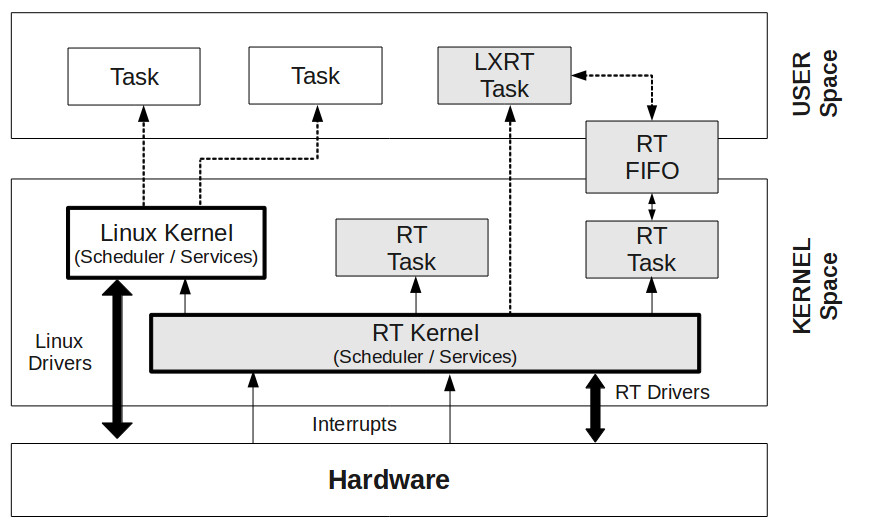
\includegraphics[width=0.95\textwidth]{./07-images/img-Ch4App/rtai-architecture-on-linux.jpg}
		\caption{App4-Real Time Application Interface (RTAI) architecture on Linux}
		\label{fig:App4-rtai-architecture-on-linux.jpg}
	\end{center}
\end{figure}

There are two(2) aspects of writing software codes for CNC machines we undertook in our past projects. 
\begin{enumerate}
	\item writing C/C++ \textbf{realtime codes} using the Linux environment RTAI. Realtime for a process here means strictly meeting both its start and end deadlines. 
	
	\item writing C/C++ \textbf{parallel codes} using the multi-threading library in C++11 onwards (version 2011 and up). Parallel for two processes here means both processes run overlapping in time.
\end{enumerate}

In the next section, we provide a glimpse, or an extract of the realtime codes we wrote using RTAI libraries (written in C/C++). The RTAI library uses the prefixes (RT\_ and rt\_) exclusively, to denote constants, variables and functions that belong to its modules. The RTAI codes can intermingle with standard C/C++ codes. A few examples of RTAI codes are:\\
rt\_task\_init(...), rt\_make\_hard\_real\_time(), rt\_set\_oneshot\_mode(), rt\_set\_periodic\_mode(), rt\_task\_delete(), start\_rt\_timer(), stop\_rt\_timer(), and so on. The RTAI library is huge.
\vspace*{1\baselineskip}

RTAI programming is basically interrupt-based programming, as can be seen in the figure above. We will discuss this further in the section on literature review.
\vspace*{1\baselineskip}

In a later section, we will provide some sample parallel running C/C++ multi-threading codes that we have used in our past projects. Since, the codes are also standard C/C++ codes, they can also intermingle with RTAI codes. Similarly, we will discuss this further in the section on literature review.

\pagebreak

\subsection{App4-C/C++ Code excerpt for Real Time (RTAI)}

% ==========================================================
\lstset{basicstyle=\footnotesize, numberstyle=\tiny\color{blue}, frame=single, numbers=left, firstnumber=1, stepnumber=1, numbersep=1pt, xleftmargin=2.0em, framexleftmargin=1.5em, xrightmargin=0.0em, breaklines=true, breakatwhitespace=false, breakindent=5pt, prebreak=\space, postbreak=\space }
% ==========================================================

\begin{lstlisting}[caption={C/C++ Code excerpt for Real Time (RTAI)}, label=AC/C++ Code excerpt for Real Time (RTAI)]
// File: rtai-CNC14.c
// Date: May 05, 2018 10:04
// Author: WRY
//*
For full RTAI Ver 5.1 LOCAL DOCUMENTATION
	file:///usr/realtime/share/doc/rtai-5.1/html/api/files.html
	For <rtai.h>
	file:///usr/realtime/share/doc/rtai-5.1/html/api/rtai_8h_source.html
	For <rtai_lxrt.h>
	file:///usr/realtime/share/doc/rtai-5.1/html/api/rtai__lxrt_8h.html
*/
// =========================================================
// EXAMPLE USAGE OF RTAI FUNCTIONS (INTERRUPT-BASED)
// ========================================================= 
/*	rt_set_oneshot_mode();
	rt_set_periodic_mode();
	start_rt_timer();
	rt_request_irq_task(PARPORT_IRQ, WRY_RT_task, RT_IRQ_TASK, 1)
	rt_task_init(); 
	rt_task_make_periodic(); 
	rt_make_hard_real_time();
	rt_make_soft_real_time();
	rt_allow_nonroot_hrt();
	rt_task_delete(WRY_RT_task);
	stop_rt_timer();
*/
// Later on in program we make task periodic (change value to 0)
	int 		WRY_RT_task_status = 1;  
	static RTIME 	WRYexpected;
	static RTIME 	WRYsampling_interval;	

// SELECT REAL TIME TIMER PERIOD
// NANO SECONDS MEANS (10)^(-9) SEC PERIOD.
	static RTIME 	CNCtimer_period_ns = 1000*1000*1000; 

// SET REAL TIME RUN MODE (BOTH CANNOT BE TRUE)
	int 	WRY_set_periodic_mode = 1; // TRUE  = 1 
	int		WRY_set_one_shot_mode = 0; // FALSE = 0

// GET NANOSECOND TIME
	CNCunixtime2 = rt_get_time_ns(); 
	gettimeofday(&TASKfinish,NULL)
... and so on ;
\end{lstlisting}


\begin{enumerate}
	\item For the summary of functions we created for program entry, the standard functions invoked in  main(), please refer to the link [\ref{App4-Summary main() function C-Code listing for RTAI}] to the appendix. 

	\item For the full code listing, please refer to the link [\ref{App4-Full C-Code listing for Real Time (RTAI)}] to the appendix. 

	\item For RTAI compilation and terminal display of results on code execution, please refer to the link [\ref{App4-Full execution C/C++ code for Real Time (RTAI)}] to the appendix. 
\end{enumerate}

\pagebreak
% ================================================
\subsection{App4-CNC machine - First successful run (26 June, 2010)}

\begin{figure}[htbp]
	\begin{center}
	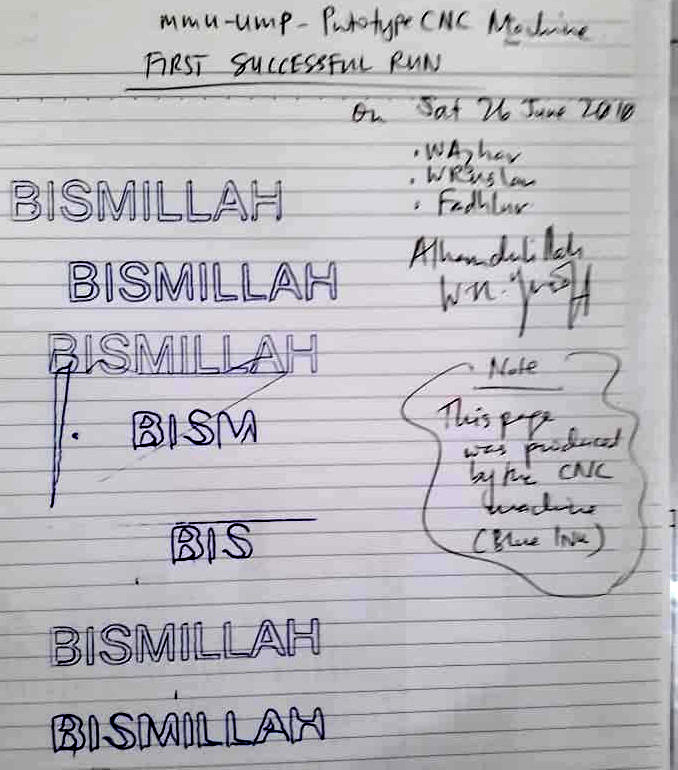
\includegraphics[width=0.80\textwidth]{./07-images/img-Ch4App/CNC-Research-machine-first-successful-run.jpg}
		\caption{App4-Witnessed first successful run CNC machine on Sat, 26 June 2010}
		\label{fig:App4-CNC-Research-machine-first-successful-run.jpg}
	\end{center}
\end{figure}

The University Malaysia Pahang (UMP) CNC Research Machine was delivered on Sat 04 December, 2009. The first successful run was conducted on Sat 26 June, 2010, less than 6 months later. The auspicious inauguration event was witnessed by three(3) team members from both UMP and MMU, as handwritten in the figure above. 
\vspace*{1\baselineskip}

The CNC drawing of BISMILLAH (meaning In The Name of Allah) took about 10 minutes to complete. The pulse generator device in use was the parallel port built-in on the motherboard of the computer. The operating system was Ubuntu 10.04 LTS 32-bit linux kernel 2.6.122 with RTAI version 2.7 modules installed. Today (as of 2018), we are using RTAI version 5.1 on our own compiled linux kernel ver 4.9.80 rtai, 64-bit configuration. 
\vspace*{1\baselineskip}

The CNC research machine was procured on a joint collaboration project between University Malaysia Pahang (UMP) and Multimedia University, Cyberjaya (MMU), in the year 2008, under the E-Science grant, Ministry of Science, Technology and Environment (MOSTE), Government of Malaysia.  

\pagebreak
% ================================================
\subsection{App4-First succesful run CNC Research Machine}

\begin{figure}[htbp]
	\begin{center}
		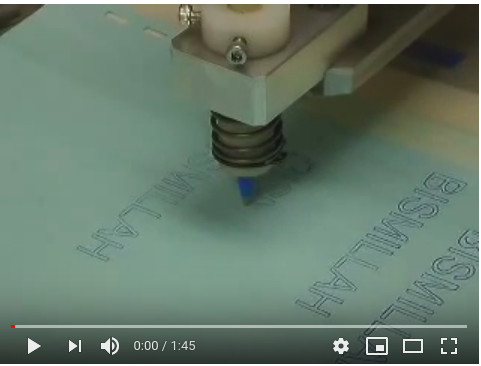
\includegraphics[width=0.75\textwidth]{./07-images/img-Ch4App/Youtube-BISMILLAH-First-Run.jpg}
		\caption{App4-BISMILLAH as first succesful run CNC Research Machine}
		\label{fig:App4-Youtube-BISMILLAH-First-Run.jpg}
	\end{center}
\end{figure}
Youtube video CNC Writing BISMILLAH (1:45 mins), link at \url{https://www.youtube.com/watch?v=0CHSr0F0bjM}, authored by wruslanhahaha, and published on Jun 5, 2011.

\subsection{App4-Pulsing both X-Y axes simultaneously}

\begin{figure}[htbp]
	\begin{center}
		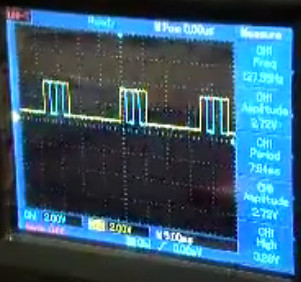
\includegraphics[width=0.43\textwidth]{./07-images/img-Ch4App/Pulsing-both-X-Y-axes-simultaneously.jpg}
		\caption{App4-Pulsing both X(blue) and Y(yellow) axes simultaneously}
		\label{fig:App4-Pulsing-both-X-Y-axes-simultaneously.jpg}
	\end{center}
\end{figure}
Both X-axis motor and Y-axis motor are receiving electrical pulses simultaneously tracing a path on the X-Y plane. The youtube link is at \url{https://www.youtube.com/watch?v=I8IGaXkV7Qs}, (0:46 mins) by WRY, published on Feb 16, 2015.

\pagebreak
% ================================================
\subsection{App4-Result 1 - Parallel port driving CNC Machine}

\begin{figure}[htbp]
	\begin{center}
		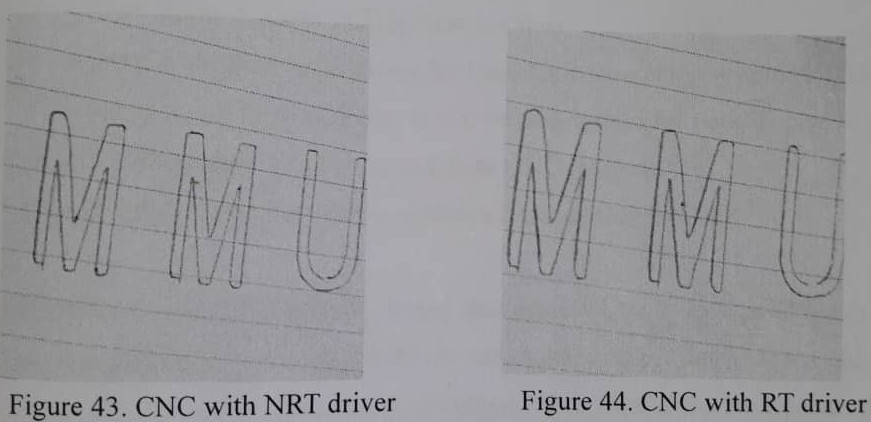
\includegraphics[width=0.80\textwidth]{./07-images/img-Ch4App/Abzal-CNC-NRT-versus-RT-Driven.jpg}
		\caption{App4-Comparison Non-Realtime (NRT) versus Realtime (RT) pulse driving.}
		\label{fig:App4-Abzal - CNC-NRT-versus-RT-Driven.jpg}
	\end{center}
\end{figure}
The two(2) figures above were drawn by the CNC Research Machine using the standard desktop parallel port as the pulse generator device for the MMU Final Year Project (Abzal-2012). The comparison was made by writing non-realtime (NRT) and realtime (RT), C/C++ CNC pulse driver program codes.

\subsection{App4-Result 2 - Arduino Due USB driving CNC Machine}

\begin{figure}[htbp]
	\begin{center}
		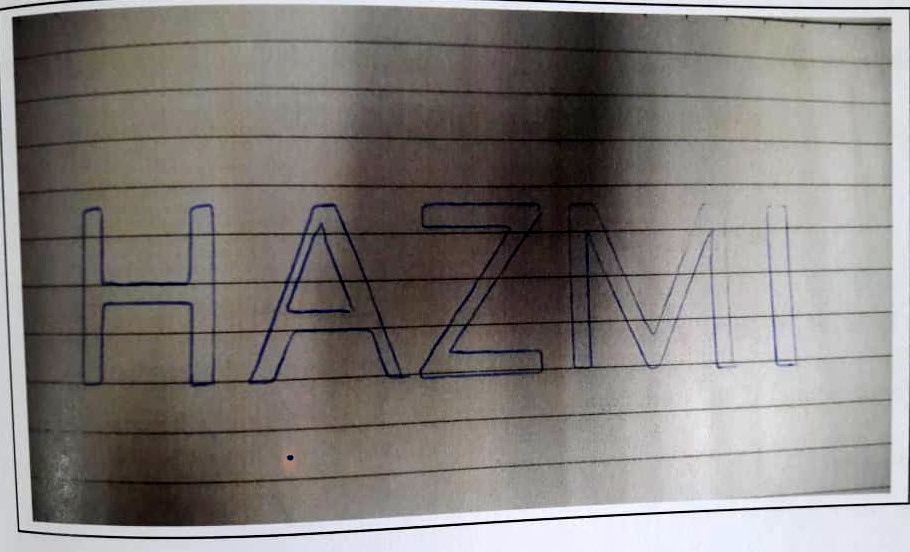
\includegraphics[width=0.80\textwidth]{./07-images/img-Ch4App/Hazmi-Arduino-Due-CNC-Driven.jpg}
		\caption{App4-Result 2 - Arduino Due USB driving CNC Research Machine}
		\label{fig:App4-Hazmi -  CNC Research Machine Arduino Due drawing HAZMI}
	\end{center}
\end{figure}
The figure above was drawn by the CNC Research Machine using the Arduino Due USB board as the pulse generator device for the MMU Final Year Project (Hazmi-2014).

\pagebreak
% ================================================
\subsection{App4-Result 3 - FPGA USB board driving CNC Machine}

\begin{figure}[htbp]
	\begin{center}
		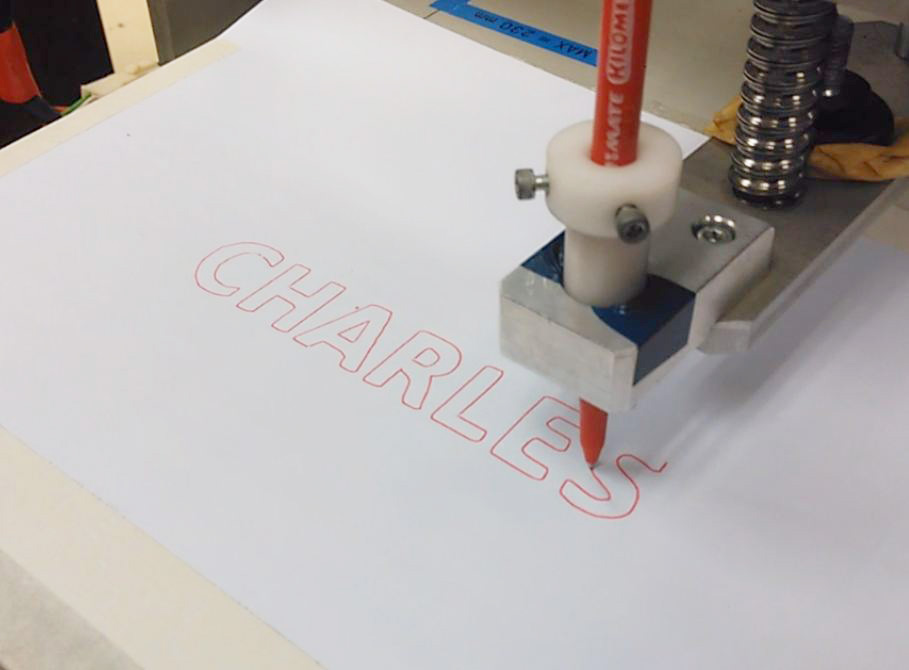
\includegraphics[width=0.80\textwidth]{./07-images/img-Ch4App/cnc-drawing-result-CHARLES.jpg}
		\caption{App4-Result 3 - FPGA USB driving CNC Research Machine}
		\label{fig:App4-Charles - CNC Research Machine FPGA drawing CHARLES}
	\end{center}
\end{figure}
The figure above was drawn by the CNC Research Machine using the Digilent Nexsys3 Spartan6 Xilinc USB Extension Board as the pulse generator device for the MMU Final Year Project (Charles-2015). Youtube link at \url{https://www.youtube.com/watch?v=3GuhE5dlcYk}, Charles Teh, published on Feb 15, 2016. 

\subsection{App4-Youtube video LINKS made for CNC Machine}

Listed below are some of the Youtube video links for the CNC Research Machine in operation. The videos are still available as at time of this writing.

\begin{enumerate}
	\item CNC Jogging Test (4:00 mins)\\ 
		\url{https://www.youtube.com/watch?v=gvlKlqfEXro}\\
		Charles Teh, published on Oct 1, 2015.
		
	\item FPGA USB Communication Test (1:33 mins)\\
		\url{https://www.youtube.com/watch?v=9kf__vntpq4}\\
		Charles Teh, published on Oct 22, 2015.
		
	\item USB Data Streaming to FPGA Test (0:58 mins)\\
		\url{https://www.youtube.com/watch?v=VvAyLqt_wLQ}\\
		Charles Teh, published on Jan 28, 2016.
		
	\item Tracing Bismillah in Arabic using LinuxCNC (4:28 mins)\\
		\url{https://www.youtube.com/watch?v=cSgsf9p9wWs&feature=youtu.be}\\
		Rajeef Selvaraja, published on Apr 10, 2015.	

\end{enumerate}

\pagebreak
% ================================================
\subsection{App4-Result 4 - Raspberry Pi-3 SBC on CNC machine}

\begin{figure}[htbp]
	\begin{center}
		
\includegraphics[width=1.00\textwidth]{./07-images/img-Ch4App/Success-drawing-Proton.jpg}
		\caption{App4-Raspberry Pi 3 SBC driving CNC Research machine}
		\label{fig:App4-Hafetzy - Raspberry Pi 3 SBC driving CNC Research machine}
	\end{center}
\end{figure}
The figure above was drawn by the CNC Research Machine using the Raspberry Pi 3 Single Board Computer (SBC) board as the pulse generator device for the MMU Final Year Project (Hafetzy-2017).

\pagebreak
% ================================================
\subsection{App4-Display pulses Counter-Clock-Wise (CCW) rotation}

\begin{figure}[htbp]
	\begin{center}
		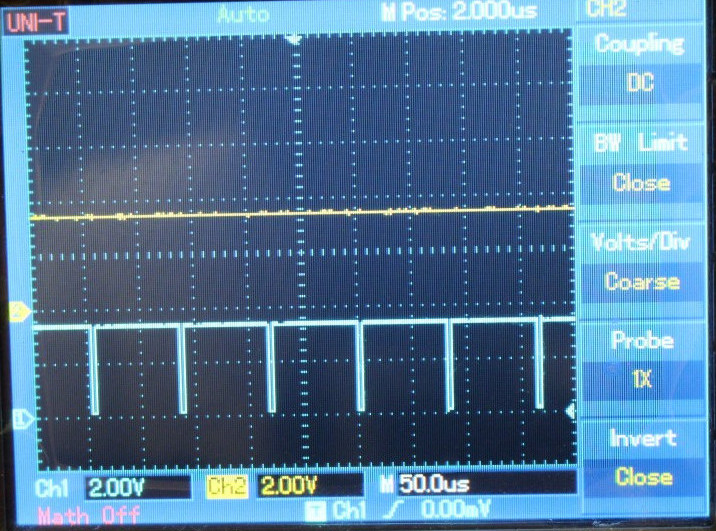
\includegraphics[width=0.65\textwidth]{./07-images/img-Ch4App/pulsing-for-CCW-motor-rotation.jpg}
		\caption{App4-Display pulses Counter-Clock-Wise (CCW) motor rotation}
		\label{fig:App4-pulsing-for-CCW-motor-rotation.jpg}
	\end{center}
\end{figure}
For motor counter-clock-wise rotation direction, yellow signal line is +5 volts above.

\subsection{App4-Display pulses Clock-Wise (CW) motor rotation}

\begin{figure}[htbp]
	\begin{center}
		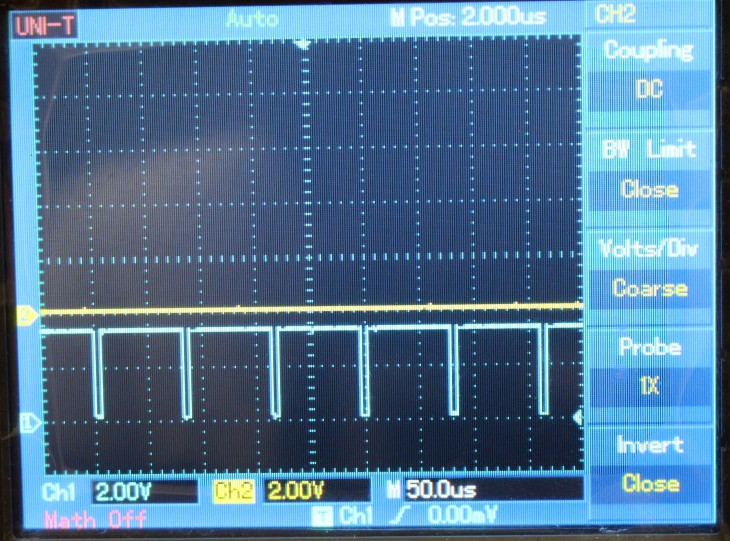
\includegraphics[width=0.65\textwidth]{./07-images/img-Ch4App/pulsing-for-CW-motor-rotation.jpg}
		\caption{App4-Display pulses Clock-Wise (CW) motor rotation}
		\label{fig:App4-pulsing-for-CW-motor-rotation.jpg}
	\end{center}
\end{figure}
For motor clock-wise rotation direction, yellow signal line is 0 volts above.

\pagebreak
% ================================================
\subsection{App4-Connection for Nexsys3 Spartan6 Xilinc USB Board}

\begin{figure}[htbp]
	\begin{center}
		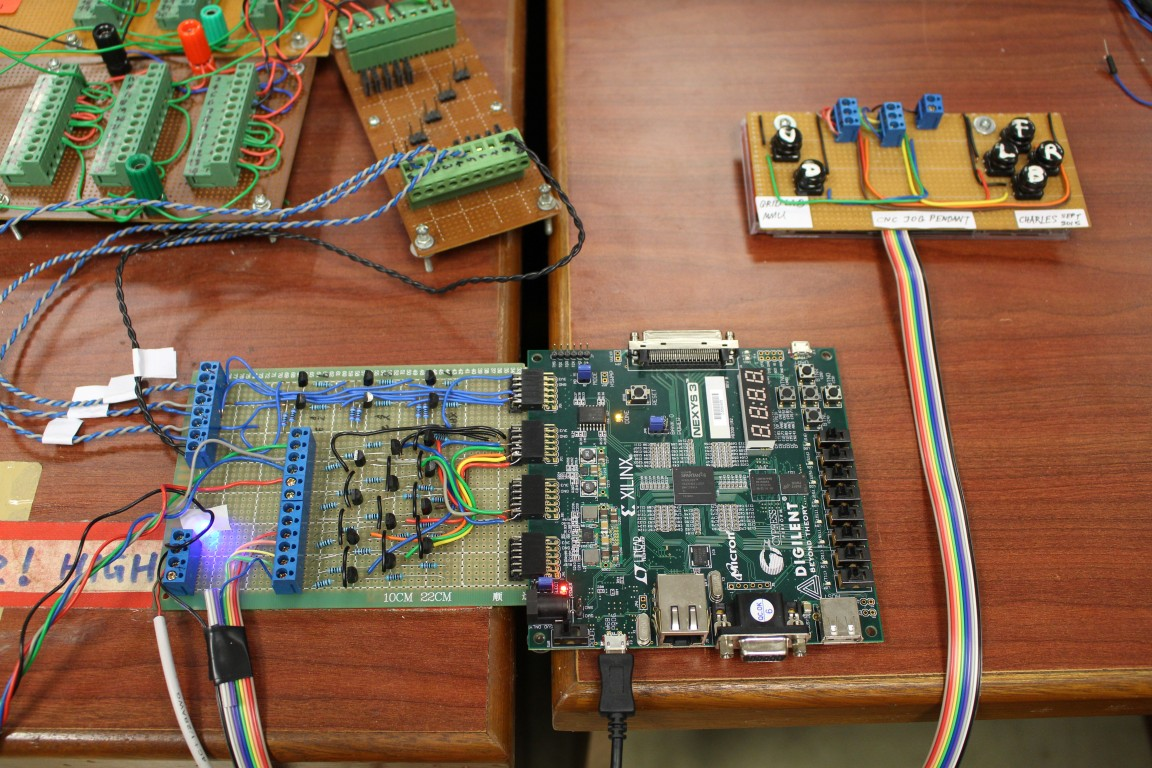
\includegraphics[width=0.95\textwidth]{./07-images/img-Ch4App/connection-setup-Nexsys3-Spartan6-Xilinc-board.jpg}
		\caption{App4-Connection setup for Digilent Nexsys3 Spartan6 Xilinc board}
		\label{fig:App4-connection-setup-Nexsys3-Spartan6-Xilinc-board.jpg}
	\end{center}
\end{figure}
The Digilent Nexys3 Spartan6 Xilinc board (bottom right) is connected via USB to a computer Notebook (bottom middle cable). The Digilent board is connected to the interface board (bottom left), which is then connected to the CNC Research Machine through a mini break-out board (top middle). The mini break-out board then connects to the servo-driver via the board (top left). A manual control switch board, called the pendant (top right), can manually drive the pen in the X-Y directions simultaneously on the CNC Research Machine, for homing or initialization tasks. 

\subsection{App4-Oscilloscope 3.3 volts pulses for CW motor rotation}

\begin{figure}[htbp]
	\begin{center}
		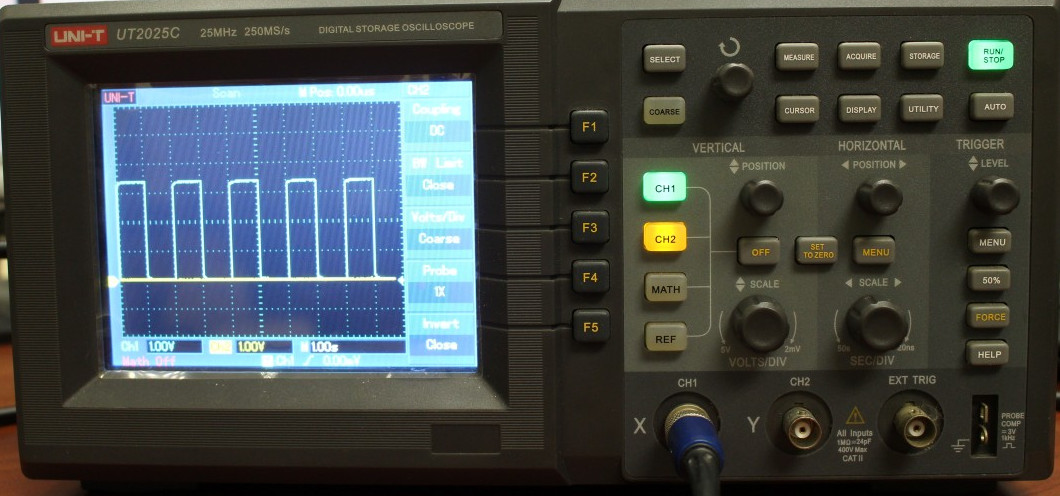
\includegraphics[width=0.62\textwidth]{./07-images/img-Ch4App/pulsing-3-3v-display-on-2-channel-oscilloscope.jpg}
		\caption{App4-Pulsing 3.3 volts display on a 2-channel digital capture oscilloscope}
		\label{fig:App4-pulsing-3.3v-display-on-2-channel-oscilloscope.jpg}
	\end{center}
\end{figure}


\pagebreak
% ================================================
\subsection{App4-G-Code versus CNC Signal file}

\begin{figure}[htbp]
	\begin{center}
		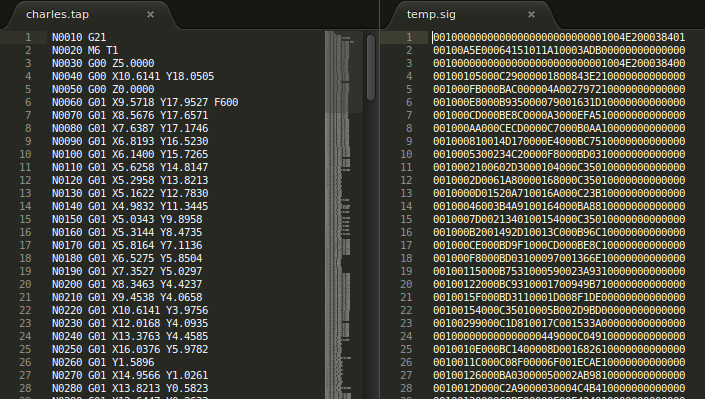
\includegraphics[width=1.00\textwidth]{./07-images/img-Ch4App/gcode-left-to-signal-file-right.jpg}
		\caption{App4-G-Code (left) versus CNC Signal file (right)}
		\label{fig:App4-gcode-left-to-signal-file-right.jpg}
	\end{center}
\end{figure}

\subsection{App4-Two inputs lines for motor CW and CCW rotations}

\begin{figure}[htbp]
	\begin{center}
		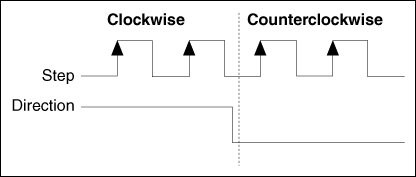
\includegraphics[width=0.95\textwidth]{./07-images/img-Ch4App/two-inputs-motor-signals-pulse-and-direction-CW-and-CCW.jpg}
		\caption{App4-Two inputs signal lines to servo-motor (CW and CCW) rotations}
		\label{fig:App4-two-inputs-motor-signals-pulse-and-direction-CW-and-CCW.jpg}
	\end{center}
\end{figure}
To drive each one of the CNC Research machine servo-driver and servo-motor pair, two(2) signal cables are required. One cable called STEP, provide a train of pulses at a rate corresponding to the pulse frequency (feedrate) to drive (rotation speed) of the electrical motor. Another cable, called DIRECTION, provides only one of two signal (high/low) states, and that state determines the direction of motor rotation (CW/CCW) or (clockwise/counterclockwise) For example high means CCW, low means CW. This is hardware dependent. 

\pagebreak
% ================================================
\subsection{App4-Acceptance delivery of UMP CNC Research Machine}

\begin{figure}[htbp]
	\begin{center}
		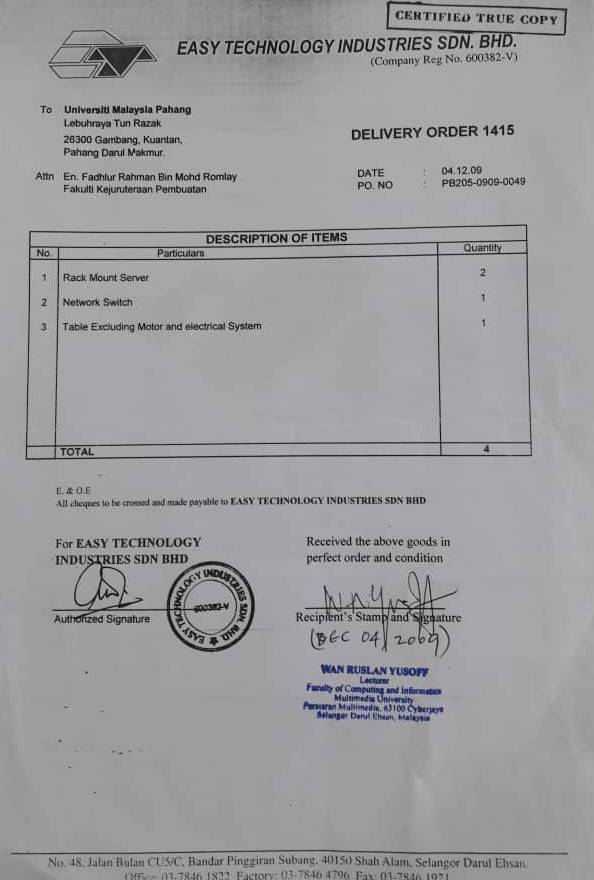
\includegraphics[width=0.75\textwidth]{./07-images/img-Ch4App/Received-Delivery-of-UMP-CNC-Research-Machine.jpg}
		\caption{App4-Acceptance of UMP CNC Research Machine on Sat, 04 Dec 2009}
		\label{fig:App4-Received-Delivery-of-UMP-CNC-Research-Machine.jpg}
	\end{center}
\end{figure}

%% ===============================================
